\chapter{VaR and Its Robust Formulation}

In the preceding chapters, we observed several limitations of the mean-variance framework such as sensitivity to errors in data as well as in the estimation of mean and variance of the underlying distribution. Furthermore, another criticism usually associated with the mean-variance setup is the use of standard deviation as a measure of risk. On the other hand, from a practitioners' point of view, the upside and downside risk cannot be perceived in the same way, because most of the times, the upside risk can improve the overall performance of the portfolio whereas the downside fluctuation usually brings impactful losses. Variance is not a reliable or appropriate  risk measure, if the underlying distribution is leptokurtic. In order to address these issues, models involving other measures of risk have been developed and accordingly their corresponding robust models have been studied as well. In the forthcoming chapters, we will elaborately discuss some of the most widely measures of risk like Value at Risk (VaR) and Conditional Value at Risk (CVaR) and also study their corresponding robust worst case formulations. 

\section{Introduction}
In this chapter, we start with the definition of VaR and formulate the optimization problems associated with VaR. Furthermore, we incorporate separable uncertainty set to model the worst case formulation. Next, we analyze and compare the performance of both VaR and Worst case VaR (WVaR) with respect to S\&P BSE 30 and S\&P BSE 100. Finally, we conclude with relevant insightful comments and conclusions.


\section{Value at Risk (VaR)}
Unlike the mean-variance setup, VaR framework takes into account the probability of losses \cite{var96}. Ghaoui et al. \cite{ghaoui03} defined VaR as the minimum value of $\gamma$ such that the probability of loss exceeding $\gamma$ is less than $\epsilon$. Accordingly, the VaR is defined as,
\begin{equation}
\begin{split}
V(\mathbf{x}) = \min \, \left\{ \gamma :  \, P\left\{\gamma \leq -r(\mathbf{x},\boldsymbol{\mu})\right\} \leq \epsilon \right\},  \\
\end{split}
\label{fig:var_basic}
\end{equation}
where $\epsilon \in (0,1)$. When we deal with mean-variance setup, only the mean and the variance \textit{i.e., the first and the second moments} of the asset returns are required, but in the VaR framework, the knowledge of the entire distribution is necessary for the computation part. If the underlying distribution is Gaussian with the moments' pair as ($\hat{\boldsymbol{\mu}}$, $\Sigma$), then VaR can be computed via the following analytical form:
\begin{equation}
\begin{split}
V(\mathbf{x}) = \kappa(\epsilon)\sqrt{\mathbf{x}^{\top}\Sigma \mathbf{x}} - \hat{\boldsymbol{\mu}}^{\top}\mathbf{x},
\end{split}
\label{eqn:kappa_eqn}
\end{equation}
where $\kappa(\epsilon) = -\Phi^{-1}(\epsilon)$ with $\Phi(z)$ representing the cumulative distribution for standard normal random variable. In practice, the value of the $\kappa(\epsilon)$ can be determined only if the cumulative distribution function of the underlying distribution is known apriori. However, if the distribution is unknown, then we have to rely on the Chebyshev's inequality. The bound (upper) obtained due to Chebyshev's only requires the knowledge of the first two moments' pair. We call a bound to be exact if the upper bound is attained. If not, we use the bound given by Bertsimas and Popescu \cite{bert05} \textit{i.e.,} $\displaystyle{ \kappa(\epsilon) = \sqrt{\frac{1-\epsilon}{\epsilon}}}$. Finally, we formulate the generalised VaR as follows:
\begin{equation}
\begin{split}
\min \, \kappa(\epsilon)\sqrt{\mathbf{x}^{\top}\Sigma \mathbf{x}} - \hat{\boldsymbol{\mu}}^{\top}\mathbf{x} \quad \text{subject to } \quad \mathbf{x} \in \mathcal{X},
\end{split}
\label{fig:var_general}
\end{equation}
where $\kappa(\epsilon)$ is an appropriate factor of risk chosen in accordance with the underlying distribution of asset returns and $\mathcal{X} = \left\{ \mathbf{x} : \mathbf{x}^{\top}\mathbf{1} = 1 \text{ and } \mathbf{x} \geq 0 \right\}$. The function $V(\mathbf{x})$ is convex and the global optimum can be obtained using techniques like interior-point methods and second order cone programming (SOCP).

Though VaR takes probability of losses into account, it has its own limitations. For the computation part, it requires the knowledge of the whole distribution. The computation also involves high dimensional numerical integration which may not be tractable at times and also there hasn't been an extensive research on methods using Monte Carlo simulations \cite{var96} for the design of the portfolio. Black and Litterman \cite{Black}, Pearson and Ju \cite{ju98} discussed the issues regarding the computational difference between the true VaR and the calculated VaR and determined that the error in the computation of the VaR can be attributed to errors in the estimation of the first and second moments of the asset returns.
% This can be viewed as following: For standardised normal random variable, $-\Phi^{-1}(\epsilon)$ represents the value in the upper tail of the distribution after which the area under the dsitribution is $\epsilon$. The same value for a normally distributed random variable with moments' pair as ($\hat{\boldsymbol{\mu}}$, $\Sigma$) is $\hat{\boldsymbol{\mu}}{\top}w - \kappa(\epsilon)\sqrt{w^{\top}\Sigma w}$ but this value is in upper tail. As the losses are negative, we take the negative of the value which is the desired result.

\section{Worst Case VaR}
The concept of worst-case VaR not only allows for approaching the solution in a more tractable way, but also relaxes the assumptions on the information known to us apriori. Here, we assume that only partial information about the underlying distribution is known. We also assume that the distribution of the asset returns belong to a family of allowable probability distributions $\mathcal{P}$ \cite{ghaoui03}. For example, given component wise bounds of ($\hat{\boldsymbol{\mu}}$,  $\Sigma$), $\mathcal{P}$ could comprise of normally distributed random variables with $\hat{\boldsymbol{\mu}}$ and $\Sigma$ as the moments' pairs. 

Given a probability (confidence) level $\epsilon$, the worst-case VaR can be formulated as 
\begin{equation}
\begin{split}
V_{\mathcal{P}}(\mathbf{x}) = \min \, \left\{\gamma : \, \sup_{P \in \mathcal{P}} P\left\{\gamma \leq -r(\mathbf{x},\boldsymbol{\mu})\right\} \leq \epsilon \right\},
\end{split}
\label{fig:wc_var_basic}
\end{equation}
and accordingly, the robust formulation can be written as 
\begin{equation}
\begin{split}
V_{\mathcal{P}}^{\text{opt}}(\mathbf{x}) = \min \, V_{\mathcal{P}}(\mathbf{x}) \quad \text{subject to} \quad \mathbf{x} \in \mathcal{X}, 
\end{split}
\label{fig:wc_var_general}
\end{equation}

The above optimization problems can be computed by a semi-definite programming (SDP) problem which again uses the above mentioned interior-point methods. We deal with the high dimensional problems by using bundle methods which are mainly used for large-scale (sparse) problems.

\subsection{Polytopic Uncertainty}

Motivated by the work of separable uncertainty sets by T{\"u}t{\"u}nc{\"u} and Koenig \cite{tutuncu}, one can view the robust formulation given by Ghaoui et al. \cite{ghaoui03} in case of Polytopic uncertainty, as a robust formulation of WVaR involving separable uncertainty (section: \ref{ssec:sep}). Accordingly, the formulation of the optimization problem for worst case VaR is,
\begin{equation}
\begin{split}
\min \, \kappa(\epsilon)\sqrt{\mathbf{x}^{\top}\overline{\Sigma}\mathbf{x}} - \underline{\hat{\boldsymbol{\mu}}}^{\top}\mathbf{x} \quad \text{subject to } \quad \mathbf{x} \in \mathcal{X},
\end{split}
\label{fig:var_poly}
\end{equation}
where $\overline{\Sigma}$ and $\underline{\hat{\boldsymbol{\mu}}}$ are higher bound for covariance matrix and lower bound for the estimated mean of asset returns respectively. We obtain these values by using the Non-Parametric Bootstrap algorithm where the type of distribution is unknown. This can also be viewed as a robust formulation involving polytopic uncertainty because \say{Separable uncertainty} is a special case of \say{Polytopic uncertainty}. In case of models involving ellipsoidal uncertainty sets, the robust worst-case VaR formulation is not that trivial and such models mainly revolve around the assumption of factor models.

\section{Computational Results}
In this section, we carry out the comparative analysis on the performance of the optimal portfolios obtained when VaR (referred as \say{Base VaR} from hereon) and WVaR are incorporated as measures of risk in the robust portfolio optimization problem. We carry out the analysis in a similar fashion as we have completed for mean-variance setup. On the same lines, we use Sharpe Ratio (SR) as a metric to compare the performance of the portfolios where the annualised risk-free rate is taken as 6\% \cite{rbi}. We perform the empirical analysis for the available historical data for S\&P BSE 30 $(N = 31)$ and S\&P BSE 100 $(N = 98)$. The reason behind this setup is to observe the trends/patterns in the performance of the portfolio when the number of stocks taken into consideration for constructing the optimal portfolio are changed. Furthermore, we also analyze the performance of the portfolio when in place of real market data, simulated data with true moments' pair is fed to the robust optimization problem. We dive one step further deep in above setup and vary the number of simulations to observe the changes in the performance of the optimal portfolio with increasing the number of simulations. For the above cause, we simulate two data-sets with true moments' pair, one with exact number of samples as in the available real market data, say, $\zeta \, (\leq 1000)$ and another with a large number of samples, say 1000. We also use the same setup in order to analyze the performance of the portfolio when different type of data is taken into consideration \textit{i.e.,} real market and simulated data. For the computational part of the robust formulation, we choose $\mathcal{P}$ to be family of distribution with the first and the second moments as the true mean and variance of the historical data. As the knowledge of the distribution is unknown, we use $\kappa$ from equation (\ref{eqn:kappa_eqn}), where we only consider the values of $\epsilon$ to be in (0,0.1) \textit{i.e.,} the confidence level is greater than or equal to 90\% In the following subsections, we analyze each scenario in detail with appropriate figures and tables. We allow a slight notational abuse and refer the model which uses Base VaR/ WVaR as a measure of risk as VaR and WVaR respectively. We start our discussion with smaller number of stocks for which we obtain data from S\&P BSE 30 and accordingly compute the log returns from the asset values.


\subsection{Performance with $N=31$ Assets}
We proceed with the analysis of the performance of the portfolio when real market data is used to construct the optimal portfolio. From Figure \ref{fig:5.1} one can observe that the performance of the portfolio is better when basic definition of VaR is used in the optimization problem. The Base VaR model outperforms the WVaR model over the complete range of $\epsilon$.
\begin{figure}[!h]
\centering
\includegraphics[height=7.0cm,width=0.7\textwidth]{VaR/bse30_market/sr_cheb.eps}
\caption{Sharpe ratio plot for Base VaR and WVaR models in case of Market data (31 assets)}
\label{fig:5.1}
\end{figure}
For a better understanding of the trends, we mainly tabulated the values of Sharpe ratio for the optimal portfolios obtained with different values of $\epsilon$ in Table \ref{tab:5.1}. We can observe that the average value of Sharpe ratio is more for Base VaR model when compared to WVaR model and is obvious from the Figure \ref{fig:5.1}.

\begin{table}[!h]
\centering
\captionsetup{justification=centering}
\begin{tabular}{||c|c|c|c|c|c|c||}
\hline
$\epsilon$ & $\mu_{VaR}$ & $\sigma_{VaR}$ & $\mu_{WVaR}$ & $\sigma_{WVaR}$ & $SR_{VaR}$ & $SR_{WVaR}$\\
\hline
0.0001 & 0.000646 & 0.00522 & 0.000603 & 0.00528 & 0.0932 & 0.0839 \\
0.0201 & 0.000715 & 0.00522 & 0.00066 & 0.00529 & 0.106 & 0.0947 \\
0.0401 & 0.000744 & 0.00523 & 0.000687 & 0.0053 & 0.112 & 0.0995 \\
0.0601 & 0.000763 & 0.00523 & 0.000708 & 0.0053 & 0.115 & 0.103 \\
0.0801 & 0.000777 &0.00524 & 0.000726 & 0.00531 & 0.118 & 0.107 \\
\hline
& & & & Avg & 0.111	& 0.0998 \\
\hline
\end{tabular}
\caption{Empirical Analysis of Base VaR and WVaR models in case of Market Data (31 assets)}
\label{tab:5.1}
\end{table}

Now, we move to the domain of the simulated data. Firstly, we discuss the trends in the performance of the optimal portfolio when the number of the samples ($\zeta$) generated are same as there are in the real market data. We observe from the Figure \ref{fig:5.2} that there is hardly any difference in trends of the performance when we used $\zeta$ number of simulations when compared to the real market data. 
\begin{figure}[!h]
\centering
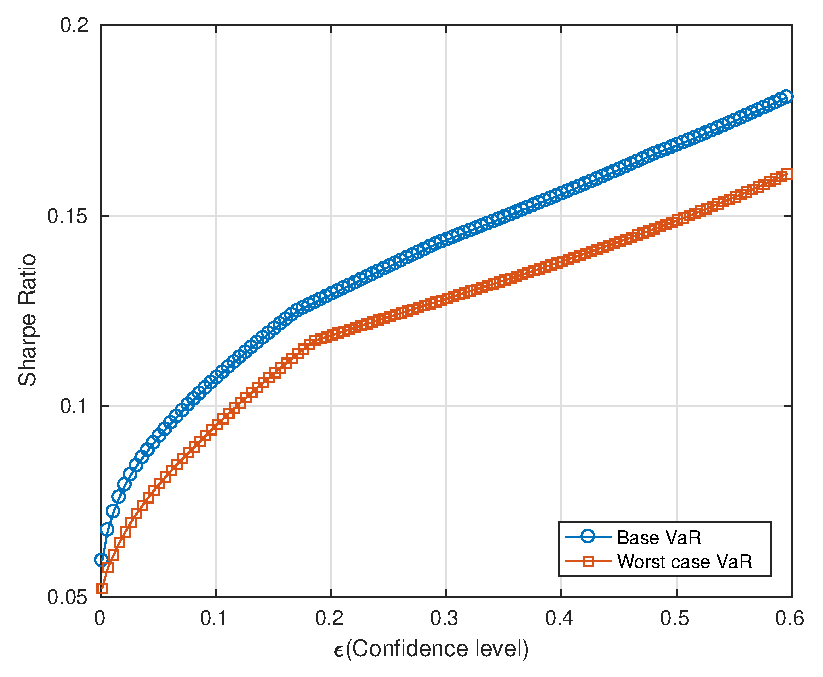
\includegraphics[height=7.0cm,width=0.7\textwidth]{VaR/bse30_simulated/sr_exact_cheb.eps}
\caption{Sharpe ratio plot for Base VaR and WVaR models in case of simulated data with $\zeta$ number of samples (31 assets)}
\label{fig:5.2}
\end{figure}
Also from Table \ref{tab:5.2}, we can observe that the Base VaR model exhibits superior performance over WVaR model on the complete range of $\epsilon$.

\begin{table}[!h]
\centering
\captionsetup{justification=centering}
\begin{tabular}{||c|c|c|c|c|c|c||}
\hline
$\epsilon$ & $\mu_{VaR}$ & $\sigma_{VaR}$ & $\mu_{WVaR}$ & $\sigma_{WVaR}$ & $SR_{VaR}$ & $SR_{WVaR}$\\
\hline
0.0001 & 0.000444 & 0.00509 & 0.000417 & 0.00519 & 0.0557 & 0.0496 \\
0.0201 & 0.000562 & 0.0051 & 0.000506 & 0.0052 & 0.0788 & 0.0665 \\
0.0401 & 0.00061 & 0.00511 & 0.000554 & 0.00521 & 0.0881 & 0.0756 \\
0.0601 & 0.000647 & 0.00512 & 0.000592 & 0.00522 & 0.0953 & 0.0828 \\
0.0801 & 0.000681 & 0.00513 & 0.000625 & 0.00523 & 0.102 & 0.089 \\
\hline
& & & & Avg & 0.0884 & 0.0765 \\
\hline
\end{tabular}
\caption{Empirical Analysis of Base VaR and WVaR models in case of simulated data with $\zeta$ number of samples (31 assets)}
\label{tab:5.2}
\end{table}

Since the model with $\zeta$ number of samples, results in the same trends as in the real market data, we now consider the case where we simulated larger number of samples, say 1000 with a justification, that larger the number of samples, less is the difference between true moments' pair with their computed counterparts.

In this case, from Figure \ref{fig:5.3}, we observe that the WVaR model delivers better performance than the Base VaR model in the $\epsilon$ interval of (0, 0.04]. So, for more conservative investors, WVaR model will benefit more than the corresponding VaR model.
\begin{figure}[!h]
\centering
\includegraphics[height=7.0cm,width=0.7\textwidth]{VaR/bse30_simulated/sr_1000_cheb.eps}
\caption{Sharpe ratio plot for Base VaR and WVaR models in case of simulated data with 1000 samples (31 assets)}
\label{fig:5.3}
\end{figure}
In the Table \ref{tab:5.3}, one can cross-check the observation made above, the WVaR model performs better than Base VaR model in the interval (0, 0.04] of $\epsilon$. However, the average values remains almost equal because after the interval (0, 0.04], the Base VaR model outperforms the WVaR model. So, we conclude that in this case, both Base VaR and WVaR models are indifferent from the perspective of a rational investor.
\begin{table}[!h]
\centering
\captionsetup{justification=centering}
\begin{tabular}{||c|c|c|c|c|c|c||}
\hline
$\epsilon$ & $\mu_{VaR}$ & $\sigma_{VaR}$ & $\mu_{WVaR}$ & $\sigma_{WVaR}$ & $SR_{VaR}$ & $SR_{WVaR}$\\
\hline
0.0001 & 0.000587 & 0.00507 & 0.000605 & 0.0051 & 0.0842 & 0.0873 \\
0.0201 & 0.000636 & 0.00508 & 0.000645 & 0.0051 & 0.0937 & 0.0951 \\
0.0401 & 0.00066 & 0.00508 & 0.000663 & 0.00511 & 0.0984 & 0.0986 \\
0.0601 & 0.00068 & 0.00509 & 0.000678 & 0.00511 & 0.102 & 0.101 \\
0.0801 & 0.000694 & 0.00509 & 0.000691 & 0.00512 & 0.105 & 0.104 \\
\hline
& & & & Avg & 0.0987 & 0.0989 \\
\hline
\end{tabular}
\caption{Empirical Analysis of Base VaR and WVaR models in case of simulated data with 1000 samples (31 assets)}
\label{tab:5.3}
\end{table}
We now extend the same type of analysis for a larger set of stocks for which we obtain data from S\&P BSE 100 ($N = 98$).

\subsection{Performance with $N=98$ Assets}
In the same lines, we begin our discussion of analyzing the performance of the Base VaR and WVaR models when real market data from S\&P BSE 100 is taken into consideration. We present the empirical results in Figure \ref{fig:5.4} and tabulate the observations in Table \ref{tab:5.4}. One can observe from the plot that the WVaR model exhibits superior performance in comparison to the corresponding Base VaR model on the entire range of $\epsilon$. This observation can also be quantitatively justified by Table \ref{tab:5.4} where the Sharpe Ratios of the portfolios obtained from WVaR model is greater than that of Base VaR model.
\begin{figure}[!h]
\centering
\includegraphics[height=7.0cm,width=0.7\textwidth]{VaR/bse100_market/sr_cheb.eps}
\caption{Sharpe ratio plot for Base VaR and WVaR models in case of market data (98 assets)}
\label{fig:5.4}
\end{figure}

\begin{table}[!h]
\centering
\captionsetup{justification=centering}
\begin{tabular}{||c|c|c|c|c|c|c||}
\hline
$\epsilon$ & $\mu_{VaR}$ & $\sigma_{VaR}$ & $\mu_{WVaR}$ & $\sigma_{WVaR}$ & $SR_{VaR}$ & $SR_{WVaR}$\\
\hline
0.0001 & 0.000667 & 0.00484 & 0.00071 & 0.00496 & 0.105 & 0.111 \\ 
0.0201 & 0.000713 & 0.00485 & 0.000755 & 0.00497 & 0.114 & 0.12 \\
0.0401 & 0.000735 & 0.00485 & 0.000776 & 0.00498 & 0.119 & 0.124 \\
0.0601 & 0.000751 & 0.00486 & 0.000793 & 0.00499 & 0.122 & 0.127 \\
0.0801 & 0.000765 & 0.00486 & 0.000807 & 0.005 & 0.124 & 0.13 \\
\hline
& & & & Avg & 0.119 & 0.124 \\
\hline
\end{tabular}
\caption{Empirical Analysis of Base VaR and WVaR models in case of market data (98 assets)}
\label{tab:5.4}
\end{table}

The same type of trend is observed for $N=98$ stocks in the case of simulated data as well, when the number of simulations equals $\zeta$ \textit{i.e.,} the number of instances available in the real market data of S\&P BSE 100. From Figure \ref{fig:5.5} and the Table \ref{tab:5.5}, we infer that the WVaR model performs better than the Base VaR model when Sharpe ratio is used as performance measure for every $\epsilon \in$ (0,0.1).
\begin{figure}[!h]
\centering
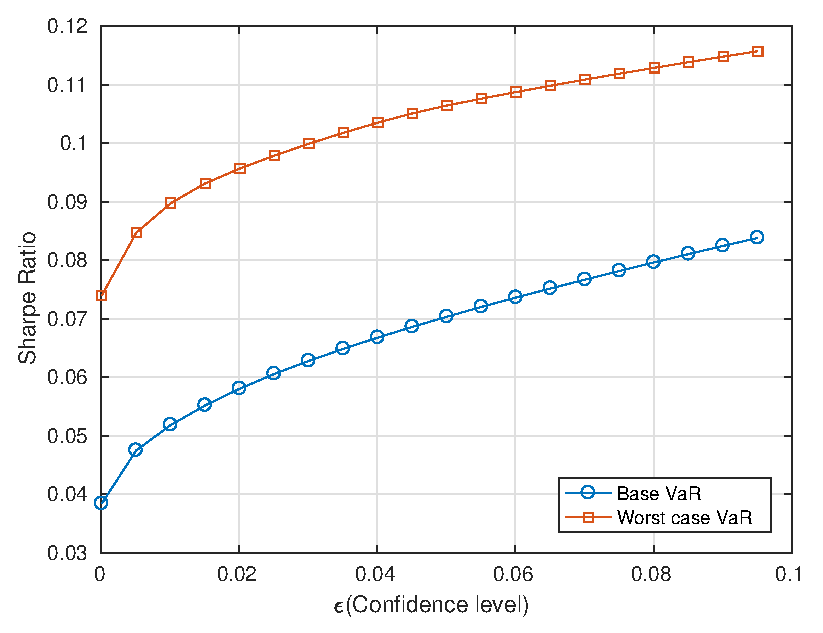
\includegraphics[height=7.0cm,width=0.7\textwidth]{VaR/bse100_simulated/sr_exact_cheb.eps}
\caption{Sharpe ratio plot for Base VaR and WVaR models in case of simulated data with $\zeta$ number of samples (98 assets)}
\label{fig:5.5}
\end{figure}

\begin{table}[!h]
\centering
\captionsetup{justification=centering}
\begin{tabular}{||c|c|c|c|c|c|c||}
\hline
$\epsilon$ & $\mu_{VaR}$ & $\sigma_{VaR}$ & $\mu_{WVaR}$ & $\sigma_{WVaR}$ & $SR_{VaR}$ & $SR_{WVaR}$\\
\hline
0.0001 & 0.000341 & 0.00471 & 0.00052 & 0.00487 & 0.0384 & 0.074 \\
0.0201 & 0.000434 & 0.00472 & 0.000629 & 0.00491 & 0.0581 & 0.0957 \\
0.0401 & 0.000475 & 0.00473 & 0.00067 & 0.00493 & 0.0668 & 0.104 \\
0.0601 & 0.000508 & 0.00473 & 0.000697 & 0.00494 & 0.0736 & 0.109 \\
0.0801 & 0.000537 & 0.00474 & 0.000719 & 0.00495 & 0.0796 & 0.113 \\ 
\hline
& & & & Avg & 0.0674 & 0.103 \\
\hline
\end{tabular}
\caption{Empirical Analysis of Base VaR and WVaR models in case of simulated data with $\zeta$ number of samples(98 assets)}
\label{tab:5.5}
\end{table}

Lastly, we consider the case where we simulated larger number of samples in order to distinguish the fluctuations in the performance of the portfolio when number of simulations are varied. Similar kind of inferences can be drawn from Figure \ref{fig:5.6} and Table \ref{tab:5.6}. The optimal portfolios obtained from the WVaR model have greater values of Sharpe ratio when compared to those obtained from Base VaR model irrespective of the value of $\epsilon$.

\begin{figure}[!h]
\centering
\includegraphics[height=7.0cm,width=0.7\textwidth]{VaR/bse100_simulated/sr_1000_cheb.eps}
\caption{Sharpe ratio plot for Base VaR and WVaR models in case of simulated data with 1000 samples (98 assets)}
\label{fig:5.6}
\end{figure}

\begin{table}[!h]
\centering
\captionsetup{justification=centering}
\begin{tabular}{||c|c|c|c|c|c|c||}
\hline
$\epsilon$ & $\mu_{VaR}$ & $\sigma_{VaR}$ & $\mu_{WVaR}$ & $\sigma_{WVaR}$ & $SR_{VaR}$ & $SR_{WVaR}$\\
\hline
0.0001 & 0.000702 & 0.00471 & 0.000822 & 0.0048 & 0.115 & 0.138 \\
0.0201 & 0.000772 & 0.00472 & 0.000897 & 0.00483 & 0.13 & 0.153 \\
0.0401 & 0.000803 & 0.00472 & 0.000931 & 0.00484 & 0.136 & 0.16 \\
0.0601 & 0.000828 & 0.00473 & 0.000959 & 0.00485 & 0.141 & 0.165 \\
0.0801 & 0.00085 & 0.00474 & 0.000982 & 0.00486 & 0.146 & 0.169 \\
\hline
& & & & Avg & 0.137 & 0.16 \\
\hline
\end{tabular}
\caption{Empirical Analysis of Base VaR and WVaR models in case of simulated data with 1000 samples (98 assets)}
\label{tab:5.6}
\end{table}